\section{Análisis y dificultades}
\subsection{Análisis}
Las mediciones son sacadas en un entorno cerrado con puertas y diferentes objetos alrededor, y el tipo de aplicación para lo que es sacado es para conocer de manera empírica como se comporta la potencia de la señal recibida mientras el receptor se va alejando del aparato transmisor de la señal en un entorno cerrado, qué tipo de perdidas se sufren y con respecto a que puede causar más perdidas por multitrayectoria.\\
Como se puede observar en la figura \ref{3m} entre 1 a 3 metros hay una puerta en el entorno, y, por otra parte, en la figura \ref{fig:grafico} desde él 1.84 metros a 1.96 metros hay una subida de decibelios, que es causada por el entorno, en este caso la puerta al estar abierta hizo que la multitrayectoria y las señales destructivas sean menores a las que había en el sector de la pared, cabe recalcar que en toda  la medición hecha no pasaban muchas personas, unas 2 o 3 como máximo a veces, lo que causaba oscilación en la potencia recibida en 7 dB.

Referente a los resultados obtenidos, estos se rigen bajo el modelo log-shadowing, como se menciona anteriormente, este modelo permite predecir la perdida de propagación en diferentes entornos, este se rige bajo la siguiente ecuación.

 \begin{figure}[H]
        \centering
        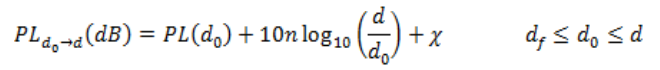
\includegraphics[width=\linewidth]{Imagenes/imagen_2022-11-08_164022665.png}
        \caption{Ecuacion log-shadowing}
        \label{log}
  \end{figure}
   Los parámetros son los siguientes
   
  \begin{itemize}
    \item \textbf{PL(d0)}:Pérdida de trayectoria en dB a una distancia d0.
   \item \textbf{PL d$>$d0}:Pérdida de trayectoria en dB a una distancia arbitraria d.
   \item \textbf{n}: Exponente de perdida
    \item \textbf{χ}: Variable aleatoria gaussiana de media cero (en dB), la desviación estándar se utiliza sólo cuando hay un efecto de sombreado. Si no hay efecto de sombreado, entonces esta variable es cero.
   
\end{itemize}
 Esta ecuación permite calcular la perdida de trayecto siempre y cuando satisfaga que la distancia inicial sea menor a la distancia de campo lejano.
  
  
  Bajo este modelo y los resultados obtenidos, se puede realizar las siguientes comparaciones en distintos escenarios.
  
  \begin{itemize}
  \item 
  
   \begin{figure}[H]
        \centering
        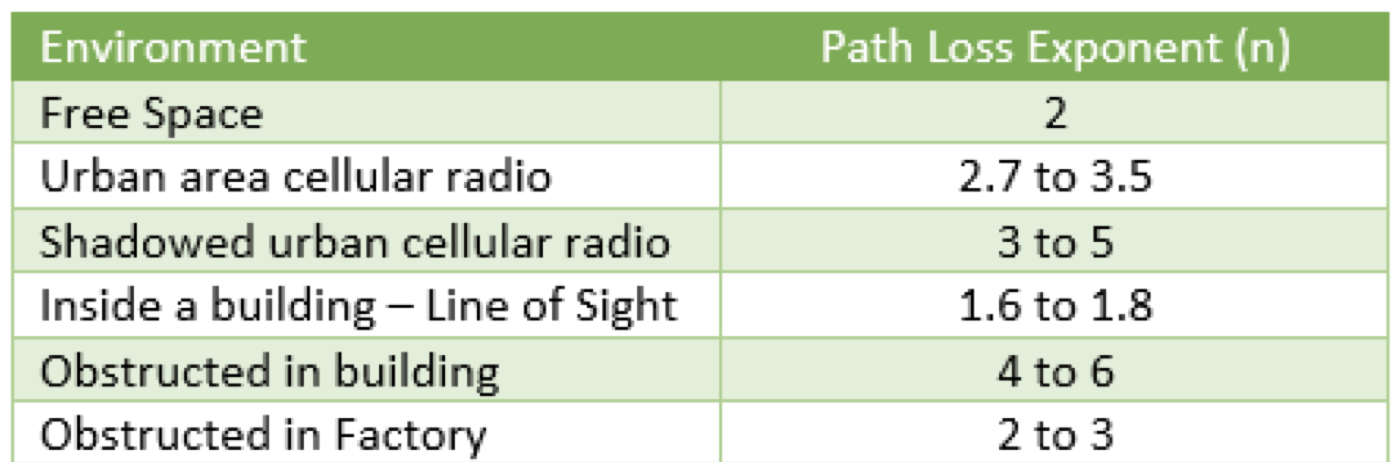
\includegraphics[width=\linewidth]{Imagenes/Captura de pantalla 2022-11-10 a la(s) 19.42.05.png}
        \caption{Tabla de exponente de perdida \cite{tabla}}
        \label{transmisor}
  \end{figure}
  
 
 
 \item En la mayoría de modelos presentes en la propagación de gran escala requieren de un proceso de simulación que se vuelve complejo para el operario, el modelo log-shadowing es una respuesta para poder simplificar tales modelos debido a que es una respuesta sistémica ya que  solo depende del exponente de perdida presentado en la comparación anterior.
  \end{itemize}
  
  \subsection{Dificultades}
  
  En la experiencia, surgieron algunas dificultades que influyeron a la hora de tomar los datos, tales dificultades  fueron:
  
  \begin{itemize}
      \item El entorno donde se ejerció la medición fue muy acotado ya que se necesito tomar las ultimas medidas en las escaleras del quinto piso de la universidad, presentando variaciones en algunos casos sumamente mayores.
      \item Durante la toma lejana de datos las personas fueron uno de los factores de variaciones muy grandes, tanto de aumento de señal como disminución de hasta $\pm$ 7dB en la muestra.
  \end{itemize}
  
  
  